\documentclass{article}

\usepackage[dvipsnames]{xcolor}
\usepackage{fancyvrb}

% redefine \VerbatimInput
\RecustomVerbatimCommand{\VerbatimInput}{VerbatimInput}%
{fontsize=\footnotesize,
 %
 frame=lines,  % top and bottom rule only
 framesep=2em, % separation between frame and text
 rulecolor=\color{Gray},
 %
%  label=\fbox{\color{Black} pict model file.txt},
 labelposition=topline,
 %
 commandchars=\|\(\), % escape character and argument delimiters for
                      % commands within the verbatim
 commentchar=\$        % comment character
}
\usepackage{listings}
\usepackage{pdfpages}
\usepackage{hyperref}
\usepackage[utf8]{inputenc}
\usepackage{babel}
\usepackage{braket}
\usepackage{indentfirst}
\usepackage{lmodern}
\usepackage{amsmath}
\usepackage{amssymb}
\usepackage{amsfonts}
\usepackage[a4paper]{geometry}
\usepackage{graphics}
\usepackage{xcolor}
\usepackage{graphicx}
\usepackage[export]{adjustbox}
\usepackage{float}
\usepackage{caption}
\usepackage{subcaption}
\usepackage{fullpage}
\usepackage{amsmath}
\usepackage{amssymb}
\usepackage{algpseudocode}
\usepackage{algorithm}
\usepackage{listings}
\usepackage{subfiles}
\usepackage[section]{placeins}
\usepackage[nottoc,numbib]{tocbibind} 
\usepackage{hyperref}
\usepackage{fancyvrb}
\usepackage{listings}
\usepackage[detect-none]{siunitx}
\sisetup{range-phrase = \text{--}}
\usepackage{xcolor}
\usepackage{multicol}
\usepackage{tikz}
\usetikzlibrary{positioning}
\captionsetup{compatibility=false}
\title{LINFO2345 - Project - Random Peer Sampling}

\begin{document}


\begin{titlepage}

     \begin{figure}[H]
        
\includegraphics[width=7cm, center]{images/Stemma_unipi.svg.png}
        \label{fig:number components}
    \end{figure}


\begin{center}
    \LARGE{UNIVERSITÀ DI PISA}
    \vspace{5mm}
    \\ \LARGE{Distributed Systems and Middleware Technologies}
\end{center}

\vspace{15mm}
\begin{center}
    {\LARGE{\bf Distributed File System with Pastry\\ \vspace{5mm}}}
    
    % Se il titolo è abbastanza corto da stare su una riga, si può usare
    
    % {\LARGE{\bf Un fantastico titolo per la mia tesi!}}
\end{center}
\vspace{20mm}

\begin{center}
    {\LARGE{{\bf Iacopo Canetta\\ \vspace{5mm}}}}
    {\LARGE{{\bf Francesco Berti\\ \vspace{5mm}}}}
\end{center}

\vspace{18mm}
\hrulefill
\\\centering{\large{ANNO ACCADEMICO 2024/2025}}

\end{titlepage}


\tableofcontents
\newpage

\section{Introduction}

This project consists in the implementation of a peer-to-peer distributed 
file storage using a distributed hash table for locating the files among the nodes. 
The distributed hash table is based on Pastry protocol.

\section{Pastry}

Pastry implements a logical ring of nodes, and each node has an ID. The files are hashed to get a key, 
and the key is used to identify which node is responsible for that file, 
checking which one has the longest common prefix. 
When a file is accessed or stored, a request is sent to the current node. 
When a node receives a request, it uses a routing table, structured as a tree, 
for finding the next hop for the request. Every time a row of the routing table is accessed, 
b bits of the prefix of the key are used to identify the correct column. If the b bits of the 
prefix are owned by the current node, the next row is visited, 
otherwise the address of the next hop is retrieved.


Whenever an address is not found or the whole table is crossed, an extra table is checked, 
called leaf set and containing the nodes with id close to the current node; 
if no node in the leaf set has a longer shared prefix with the key than the current node, 
then the current node is responsible for the file. 
This routing table, using N nodes, guarantees a maximum number of hops equal to logn.

\section{Implementation}

The implementation of the system is divided in two parts: one for the distributed file system, 
created in Erlang, and a webserver realized in Java, also thanks to the Frameworks and implementions of the Java Servlets.

\subsection{Erlang}

The Erlang code is divided in multiple modules, in order to isolate functions and keep them short enough.

\subsubsection{Util.erl, File\_handler.erl, Network.erl}

This files are created for having simple utility functions. \textit{File\_handler.erl} contains the utility functions
for dealing with files, \textit{Network.erl} contains simple functions for starting the Erlang nodes and settign the cookies, in
order to receive messages from different machines, and \textit{Util.erl} contains generic utility functions.

\subsubsection{Key\_gen.erl}

\textit{Key\_gen.erl} is the file that implements the key system for Pastry. The keys are generated hashing strings
and represented as \textit{bitstring}s; this type is chosen because it can be used for
representing streams of any number of bits, differently from the \textit{binary} type, which is exclusively for 
multiples of $8$ bits.

\textit{Bitstring}s, however, have little documentation and almost no function dedicated, so \textit{Key\_gen.erl}
also implements the functions for comparing these numbers and handling them as hexadecimals, since Pastry 
requires groups of $4$ bits for the routing.


\subsubsection{Routing.erl}

\textit{Routing.erl} represents the core of Pastry protocol, implementing the Routing Table.
The routing table is represented as a Tuple containing the TableKey, so the key of the node owning the table,
and the table. The table is a list of 32 lists, representing the rows; the single entries of the rows are 
represented by a tuple containing the hexadecimal identifying the column and the node information.

During the routing or any table modification, instead of doing the whole routing, this approach requires
of detecting the number of hexadecimals in common in the prefix, which represents the index of the row, and the 
first hexadecimal not in common, which represent the Column key.

This module contains also the functions for modifying the table and some utility functions relative to it.

\subsubsection{Leaf\_set.erl}

\textit{Leaf\_set.erl} implements the Leaf Set; the Leaf Set is represented as a Tuple of two lists, 
\textit{Left} and \textit{Right}, representing the two halves of it. The two list contain at most $L2$ elements, 
represented as tuples key-node information.


The module also offerts functions for modifying the leaf set and some utility relative to it.


\subsubsection{Node\_actions.erl}

\textit{Node\_actions.erl} implements some utility functions used by the upper modules to interact with files, 
sending messages, or broadcasting messages to lists, routing tables, or leaf sets.

The most important function is \textit{full\_route()}, which implements the full navigation of the routing table, 
and, in case of no match or it reaches the bottom, the leaf set is analyzed; the function returns the information
 of the routed node, or \textit{route\_end} if the current node is responsible for the key in input.


\subsubsection{Pastry\_actions.erl}

\textit{Pastry\_actions.erl} implements all the functions for handling the pastry requests and responses
to the other nodes in the network, plus the handling of the self messages for peridoc events.
The main functions are:

\begin{itemize}
    \item \textit{join()}: function used for responding to the \textit{join} message with the routing table row, 
    and for forwarding the message to the next node of the routing; function used by the node to join the network through another known node;
    \item \textit{join\_res\_handle()}: function used for updating the routing table and leaf set after a \textit{join\_response};
    \item \textit{exit()}: function for handling the exit of another node from the network;
    \item \textit{keepalive()}: sends keepalive to all known nodes;
    \item \textit{update\_keepalive()}: updates the keepalive of given nodes;
    \item \textit{keepalive\_res()}: responses to the keepalive to make sure that, even if a node knows another but not viceversa, 
    the one knowing still receives keepalives from the other;
    \item \textit{check\_expired\_nodes()}: checks which nodes are disconnected and updates the tables;
    \item \textit{share\_info()}: shares the info about the nodes with the known nodes.
\end{itemize}

\subsubsection{File System}

The files in this project, since it is run on a limited number of machines, are stored all in a \textit{/files} folder.
The folder contains a subfolder per each node, which contains the files owned by the node and a folder \textit{/backup}, storing a folder
per each node with their files backed up.

\subsubsection{Backup\_actions.erl}

\textit{Backup\_actions.erl} implements all the functions for sending and handling the backups.
For design choice, the backups are propagated to the whole leaf set and updated according to it.
The main functions are:

\begin{itemize}
    \item \textit{backup()}: function used for propagating a file to the leaf set for backup;
    \item \textit{backup\_res()}: function used for saving a backup sent by other node;
    \item \textit{backup\_remove()}: function used to communicate the leaf set to remove a file from backup;
    \item \textit{new\_leaf\_backup()}: function used to check if a node is added to the new leaf set, 
    and in that case it receives a backup of each file;
    \item \textit{old\_leaf\_backup()}: function used to check if a node is removed from the new leaf set, 
    and in that case it receives a message to delete the backup folder;
    \item \textit{update\_leaf\_backup()}: function used for checking in a list of nodes which
    ones entered the leaf set and which ones exited, in order to propagate or remove backups;
    \item \textit{backup\_update()}: function used to update the owner of the backups of a failed node.
    The routing is performed and, if the current node is the owner, the node moves the files to its folder,
    otherwise it forwards the request;
    \item \textit{backup\_find()}: request to find the owner of a file. If reaches the end, a \textit{backup\_found} 
    response is sent;
    \item \textit{backup\_found()}: updates the owner of a file on a \textit{backup\_found}.
\end{itemize}


\subsubsection{Web\_responses.erl}

\textit{Web\_responses.erl} implements all the functions for handling and responding to the webserver.
The main functions are:

\begin{itemize}
    \item \textit{find\_store()}: function that, given a filename, finds a storage for it using pastry routing and responds
    to the web server;
    \item \textit{store()}: function that, given a filename, it stores it on the node;
    \item \textit{find()}: function that finds a file and sends it back to the webserver;
    \item \textit{delete()}: function that, given a filename, finds for it using pastry routing, deletes it,
    and sends and ack to the web server;
    \item \textit{get\_file\_res()}: function that starts a flooding for retrieving all the names of the files
    in the network; it uses a blacklist on the \textit{Msg\_Id} for avoiding infinite flooding; 
    \item \textit{get\_files\_res\_handle()}: function that updates the list of files with the new nodes received during the flooding;
    \item \textit{all\_files\_res()}: function that responds to the webserver with the list of files;
    \item \textit{check\_expired\_blacklist()}: function called periodically for cleaning the expired entries of the blacklist.
\end{itemize}



\subsubsection{Node.erl}

\textit{Node.erl} implements a Node of the Pastry network. Nodes are started with the function \textit{start\_node()}, requiring the name
and the name of their Erlang node, in order to register their mailbox and be reachable; the new node also initializes Pastry's tables.
If \textit{Starter} is defined, the node uses the starter node to join the network, sending a join message.
At the end of the initialization, all periodical self messages are scheduled and the node enters an infinite loop, in which it just receives
messages and handles them.

\subsubsection{Controller.erl}

\textit{Controller.erl} is a simulation file used for spawning multiple nodes on one single erlang node and connecting them to the Pastry network.
This file is also responsible for creating dummy files per each node, for making the simulation more real.
Once the Controller is started, it receives in input commands from the user for spawning and killing nodes.

\subsection{Java Web Server}

\subsubsection{ErlangMessageDTO}

\textit{ErlangMessageDTO} is a java class that acts partially as a DTO for the database of this project, which is represented by Pastry.
This class is then responsible for storing all the information regarding the Erlang Messages for communicating with the distributed system, 
since the messages to the webserver have all a standard structure.

\subsubsection{ErlangMessage}

\textit{ErlangMessage} is an abstract java class that acts partially as a DAO, since it allows to access both for reads and writes in storage by using 
Erlang messages. This class implements a set of functions to call in order, used for wrapping, unwrapping, sending and receiving message, and 
for some integrity checks over the messages. This class also has two abstract methods to get and set the content of the message, which are implemented in 
classes dedicated to the single message types, since the payload of them differs partially.

\subsubsection{JavaErlangConnector}

\textit{JavaErlangConnector} is a class used to send requests from the webserver and get a response from Pastry.
After the initialization, in fact, it is necessary to simply call the dedicated function for the web request to get a 
response; these function do not return \textit{OtpErlangObjects}, in order to isolate those objects only to the layer 
directly communicating with Erlang, and to make it opaque to the webserver.

\subsubsection{WebServer}

The webserver is implemented via \textit{Java servlets} and \textit{Tomcat webserver}. There are three packages:

\begin{itemize}
    \item \textit{pastry}: contains all the servlet responsible for creating responses for the various endpoints
    \item \textit{javaerlang}: contains all classes mentioned above in the \textit{Java Web Server} section, these are used by servlets to obtain data from \textit{pastry}
    \item \textit{cleaner}: contains classes to periodically clean the \textit{files} directory in the webserver
\end{itemize}

\subsubsection{SearchServlet}
This servlet extends a \textit{HttpServlet} and it's mapped to endpoint \textit{/search}. Once a \textit{GET} request is received, the servlet opens a connection with \textit{Erlang} via \textit{JavaErlangConnector} and then calls the method \textit{find()} with the filename extracted from the URL.
\newline
If the file is found, it's saved in the \textit{files} directory of the webserver and the positive response is returned to the client in form of \textit{JSON}. The \textit{files} directory is there simply to avoid making two requests to \textit{pastry}, the first one when the client searches the file and the second one when it downloads a file. By storing the file locally, the second request is avoided.

\subsubsection{DownloadServlet}
When this servlet receives a \textit{GET} request on \textit{/download}, it will look into the \textit{"files"} directory for the file specified in the request parameter. If the file exists, it will copy the binary data in the response using the \textit{MIME} type \textit{"application/octet-stream"}. If the file does not exist, it will return a JSON with an error.

\subsubsection{UploadServlet}
This servlet responds to a \textit{PUT} request on \textit{/upload}. The request will contain the file name and the relative binary data. The servlet will extract the file name and binary data from the request and pass them to the method \textit{store} of \textit{ErlangJavaConnector}. If the file is successfully stored, it will return a \textit{201 Created} status code. If there is an error during the storage process, it will return a \textit{500 Internal Server Error} status code.

\subsubsection{DeleteServlet}
This servlet, when receiving a \textit{DELETE} request at the endpoint \textit{/delete}, will extract the file name from the request object. It will then call the \textit{delete()} method of \textit{ErlangJavaConnector} passing the extracted file name. If the file is successfully deleted, it will return a \textit{200 OK} status code. If the file does not exist or there is an error during the deletion process, it will return a \textit{404 Not Found} or \textit{500 Internal Server Error} status code, respectively.

\subsubsection{FileGetterServlet}
This servlet responds to the \textit{GET} request on endpoint \textit{/allfiles}. It will call a method to retrieve the list of all file names present in the current \textit{pastry} instance. The servlet will then return a \textit{JSON} object with an array \textit{names} containing the file names. If there is an error during the retrieval process, it will return a \textit{500 Internal Server Error} status code.

\subsubsection{JavaErlangConnector}
\textit{JavaErlangConnector} is the class used to send requests from the webserver and get a response from Pastry. The constructor takes in input various arguments:
\begin{itemize}
    \item \textit{pastryNameIn}: name of the Erlang node to connect to, it can be any Erlang node. This implies that the system can be made fault-tolerant but for simplicity the same node is always used.
    \item \textit{pastryMailBoxIn}: name of the mailbox of the previously mentioned Erlang node
    \item \textit{cookieIn}: always \textit{"pastry"}
    \item \textit{selfNameIn}: the name of the Erlang node that will be created to communicate with Pastry, it has to be unique so it includes threadId
    \item \textit{selfMailboxNameIn}: name of the mailbox for this node, it has to be unique so it includes threadId
\end{itemize}
Each time a new request is made and to fulfill that request a communication with Pastry is necessary, a new \textit{JavaErlangConnector} instance is created. This is to ensure that requests are handled concurrently, the alternative would be to use a singleton shared across the servlets which would result in a performance hit. 

\subsubsection{Cleaner}
The \textit{"files"} directory used by the webserver to temporarily hold files searched by user is cleaned by a periodic task. The period is defined in the \textit{Common} class, which also contains a method to get the full path of the \textit{files} directory in the environment which is running \textit{Tomcat}.
\newline
The \textit{cleaner} uses a \textit{ServletContextListener} to create an executor and spawn a single thread, which will run periodically, when the context is initialized. The executor will be shutdown once the context is destroyed.

\subsubsection{SemaphoreManager}
Since there are at least two threads working on the \textit{files} directory, \textit{DownloadServlet} and \textit{Cleaner}, a semaphore is used to ensure mutual exclusion when making changes to this directory. The double check lock paradigm was used since this is a multithreaded environment.

\subsection{Bash scripts}
Two scripts are used to easily deploy this application:
\begin{itemize}
    \item \textit{deploy.sh}: copies the \textit{erlang src} files as well as the \textit{WAR} file into the containers via \textit{"scp"}
    \item \textit{start.sh}: creates three terminals, connects via \textit{ssh} to the \textit{VMs}, starts \textit{erlang controllers} and \textit{tomcat}
\end{itemize}

\begin{figure}[H]
    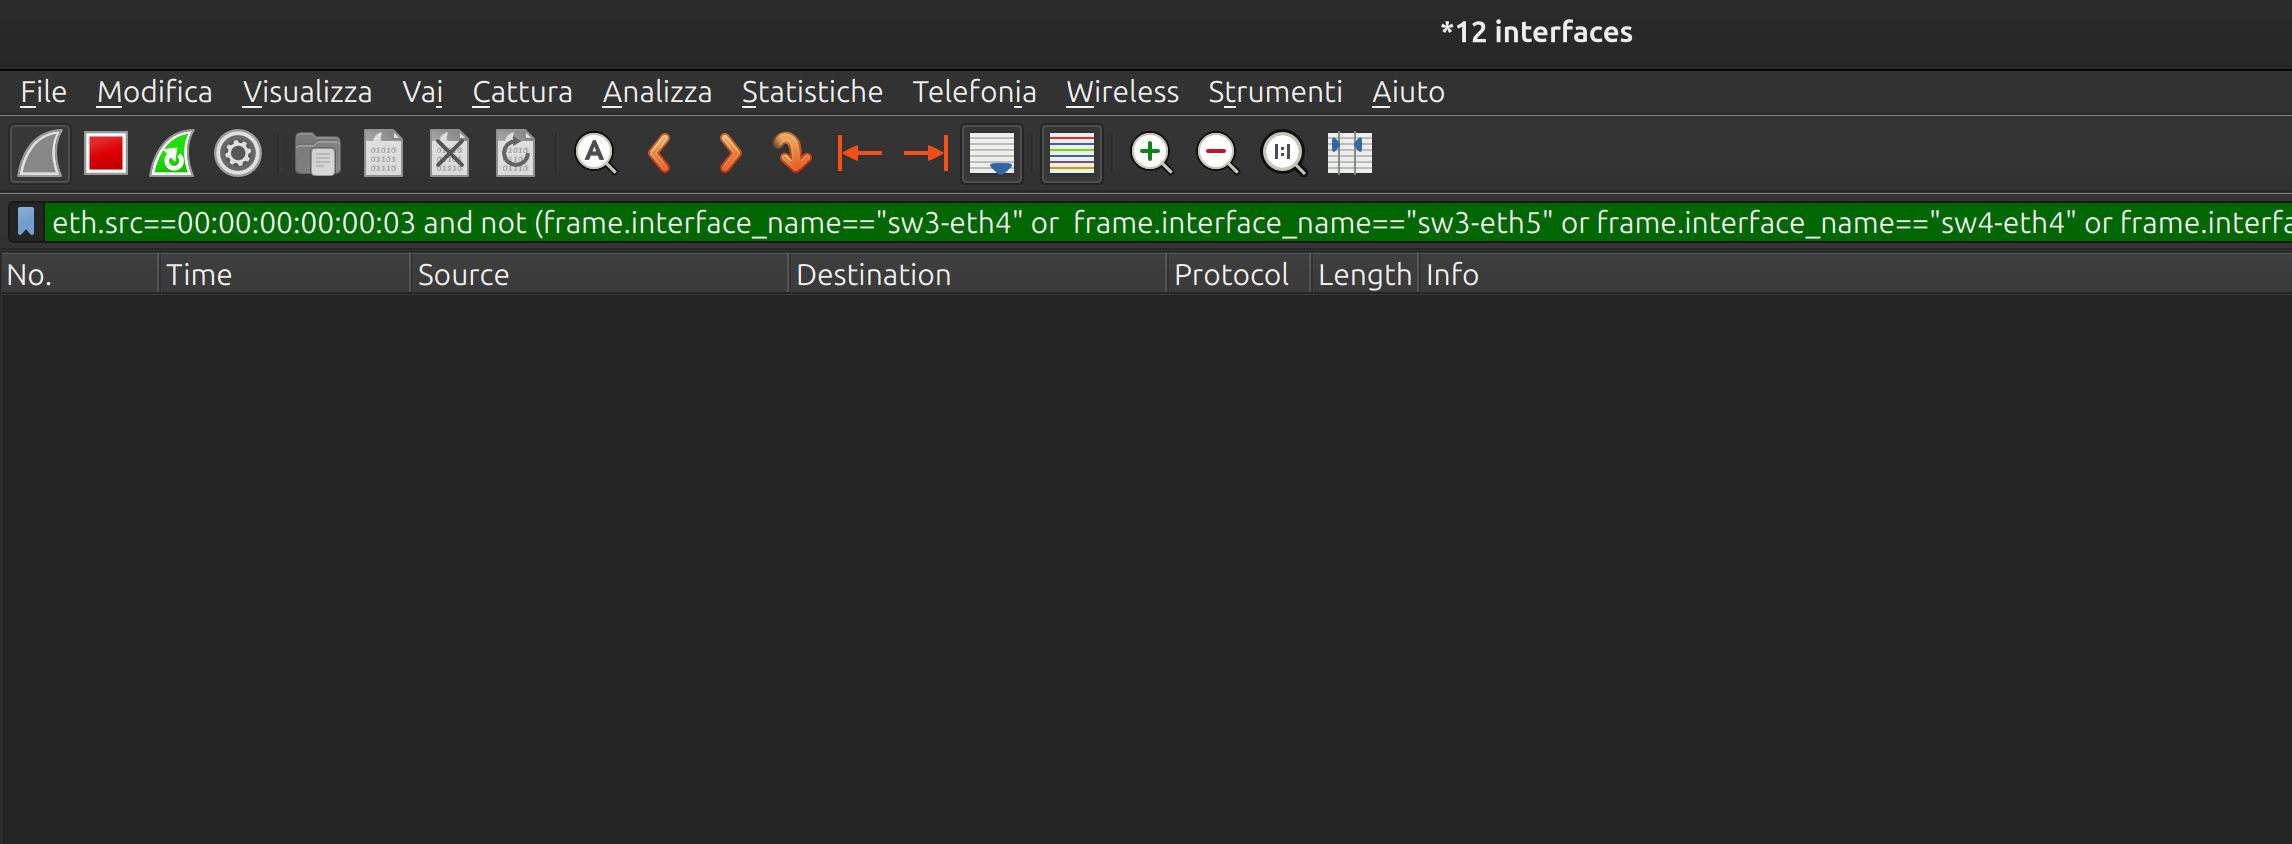
\includegraphics[width=12cm, center]{images/3-unreached.png}
    \label{fig:3unreac}
    \caption{Broadcast example 3: all other interfaces not reached}
\end{figure}


\end{document}